\documentclass{beamer}

% Setting Presentation Fonts
\usepackage{fontspec}
\setmainfont[Ligatures=TeX,BoldFont={*-Bold}]{Times-New-Roman}
\setsansfont[Ligatures=TeX,BoldFont={*-Bold}]{Times-New-Roman}
\setmonofont{Courier-New}

% For Images
\usepackage{tikz}

% New CTU fonts
\newfontfamily\technikaregular{Technika-Regular.ttf}
\newfontfamily\technikaitalic{Technika-Italic.ttf}
% Additional Technika Fonts are Available from https://campuscvut.sharepoint.com/sites/inforek-ma (after login)

% Defining Title Page Inputs

% Title
\title{\uppercase{A Brief Report on Permanent Magnet Assisted Synchronous Reluctance Motors}}

% Subtitle
%\subtitle{\uppercase{{Very long name of a presentation which is currently build in a LaTeX
%}}} % download italic technika when available

% Author
\author{Petr Zakopal}

% Supervisor
\newcommand{\SupervisorTitle}{XP14DES}
\newcommand{\SupervisorName}{}

% Opponent
\newcommand{\OpponentTitle}{}
\newcommand{\OpponentName}{}

% End of Defining Title Page Inputs

% Extra texts in FootLine and FrameTitle
\newcommand{\FootLineLeft}{\uppercase{Department of Electric Drives and Traction}}
\newcommand{\FrameTitleRight}{\uppercase{Faculty of Electrical Engineering in Prague}}

\newcommand{\cvutlogo}{
\includegraphics[scale=0.2]{src/misc/symbol_cvut_plna_verze.pdf}}


% Defining frame title based on a technika font and color
\newcommand{\techbluetitle}[1]{
    \begin{center} 
            {\fontsize{16pt}{16pt}\technikaregular {\color{ctublue}#1}}
    \end{center} 
}

% Selecting which theme to use
\usetheme{k13114}

\begin{document}

% \addtobeamertemplate{frametitle}{}{%
% \begin{tikzpicture}[remember picture,overlay]
%   \node[anchor=north west,yshift=5pt,xshift=-5pt] at (current page.north west) {\cvutlogo};
% \end{tikzpicture}}

% \addtobeamertemplate{footline}{}{%
% \begin{tikzpicture}[remember picture,overlay]
%   \node[anchor=south east,yshift=-5pt,xshift=3.5pt] at (current page.south east) {\cvutlogo};
% \end{tikzpicture}}


	\frame {
		\titlepage
	}
	\frame {
		\frametitle{Table of contents}
        %\vspace*{-2cm}
        %\techbluetitle{Structure of the report}
         {\fontsize{16pt}{16pt}\technikaregular {\color{ctublue}Structure of the report:}}
        %\vspace*{1.8cm}
        \begin{itemize}
            \item Introduction,
            \item Design,
            \item Control,
            \item Comparison to other machines,
            \item Recent research interest.
        \end{itemize}
	}
	\frame{
		\frametitle{Introduction}

        {\fontsize{14pt}{14pt}\technikaregular {\color{ctublue}PMSynRelM}}\par
        \vspace*{0.5cm}
        {\fontsize{14pt}{14pt}\technikaregular {\color{ctugrey}actively used in automotive and traction aplications}}\par
        \vspace*{0.5cm}
        {\fontsize{14pt}{14pt}\technikaregular {\color{ctugrey}control strategies based on known principles}}\par
        \vspace*{0.5cm}
        {\fontsize{14pt}{14pt}\technikaregular {\color{ctugrey}may use relatively simple mathematical model for control}}\par
	}
	\frame{
		\frametitle{Introduction}

        {\fontsize{14pt}{14pt}\technikaregular {\color{ctugrey}PMSynRelM}}\par
        \vspace*{0.5cm}
        {\fontsize{14pt}{14pt}\technikaregular {\color{ctublue}actively used in automotive and traction aplications}}\par
        \vspace*{0.5cm}
        {\fontsize{14pt}{14pt}\technikaregular {\color{ctugrey}control strategies based on known principles}}\par
        \vspace*{0.5cm}
        {\fontsize{14pt}{14pt}\technikaregular {\color{ctugrey}may use relatively simple mathematical model for control}}\par
	}
	\frame{
		\frametitle{Introduction}

        {\fontsize{14pt}{14pt}\technikaregular {\color{ctugrey}PMSynRelM}}\par
        \vspace*{0.5cm}
        {\fontsize{14pt}{14pt}\technikaregular {\color{ctugrey}actively used in automotive and traction aplications}}\par
        \vspace*{0.5cm}
        {\fontsize{14pt}{14pt}\technikaregular {\color{ctublue}control strategies based on known principles}}\par
        \vspace*{0.5cm}
        {\fontsize{14pt}{14pt}\technikaregular {\color{ctugrey}may use relatively simple mathematical model for control}}\par
	}
	\frame{
		\frametitle{Introduction}

        {\fontsize{14pt}{14pt}\technikaregular {\color{ctugrey}PMSynRelM}}\par
        \vspace*{0.5cm}
        {\fontsize{14pt}{14pt}\technikaregular {\color{ctugrey}actively used in automotive and traction aplications}}\par
        \vspace*{0.5cm}
        {\fontsize{14pt}{14pt}\technikaregular {\color{ctugrey}control strategies based on known principles}}\par
        \vspace*{0.5cm}
        {\fontsize{14pt}{14pt}\technikaregular {\color{ctublue}may use relatively simple mathematical model for control}}\par
	}
	\frame{
	    \frametitle{Design}
        \techbluetitle{Stator}
	}
	\frame{
	    \frametitle{Stator Design}
        \begin{minipage}[t]{0.30\textwidth}
            \begin{itemize}
                \item \textcolor{ctured}{Delta} winding
                \item \textcolor{ctublue}{Star} winding
                \item \textcolor{ctublue}{Star}-\textcolor{ctured}{Delta} hybrid winding
            \end{itemize}
        \end{minipage}%
        \hfill
        \begin{minipage}[t]{0.68\textwidth}
            \begin{figure}[H]
                \centering
                    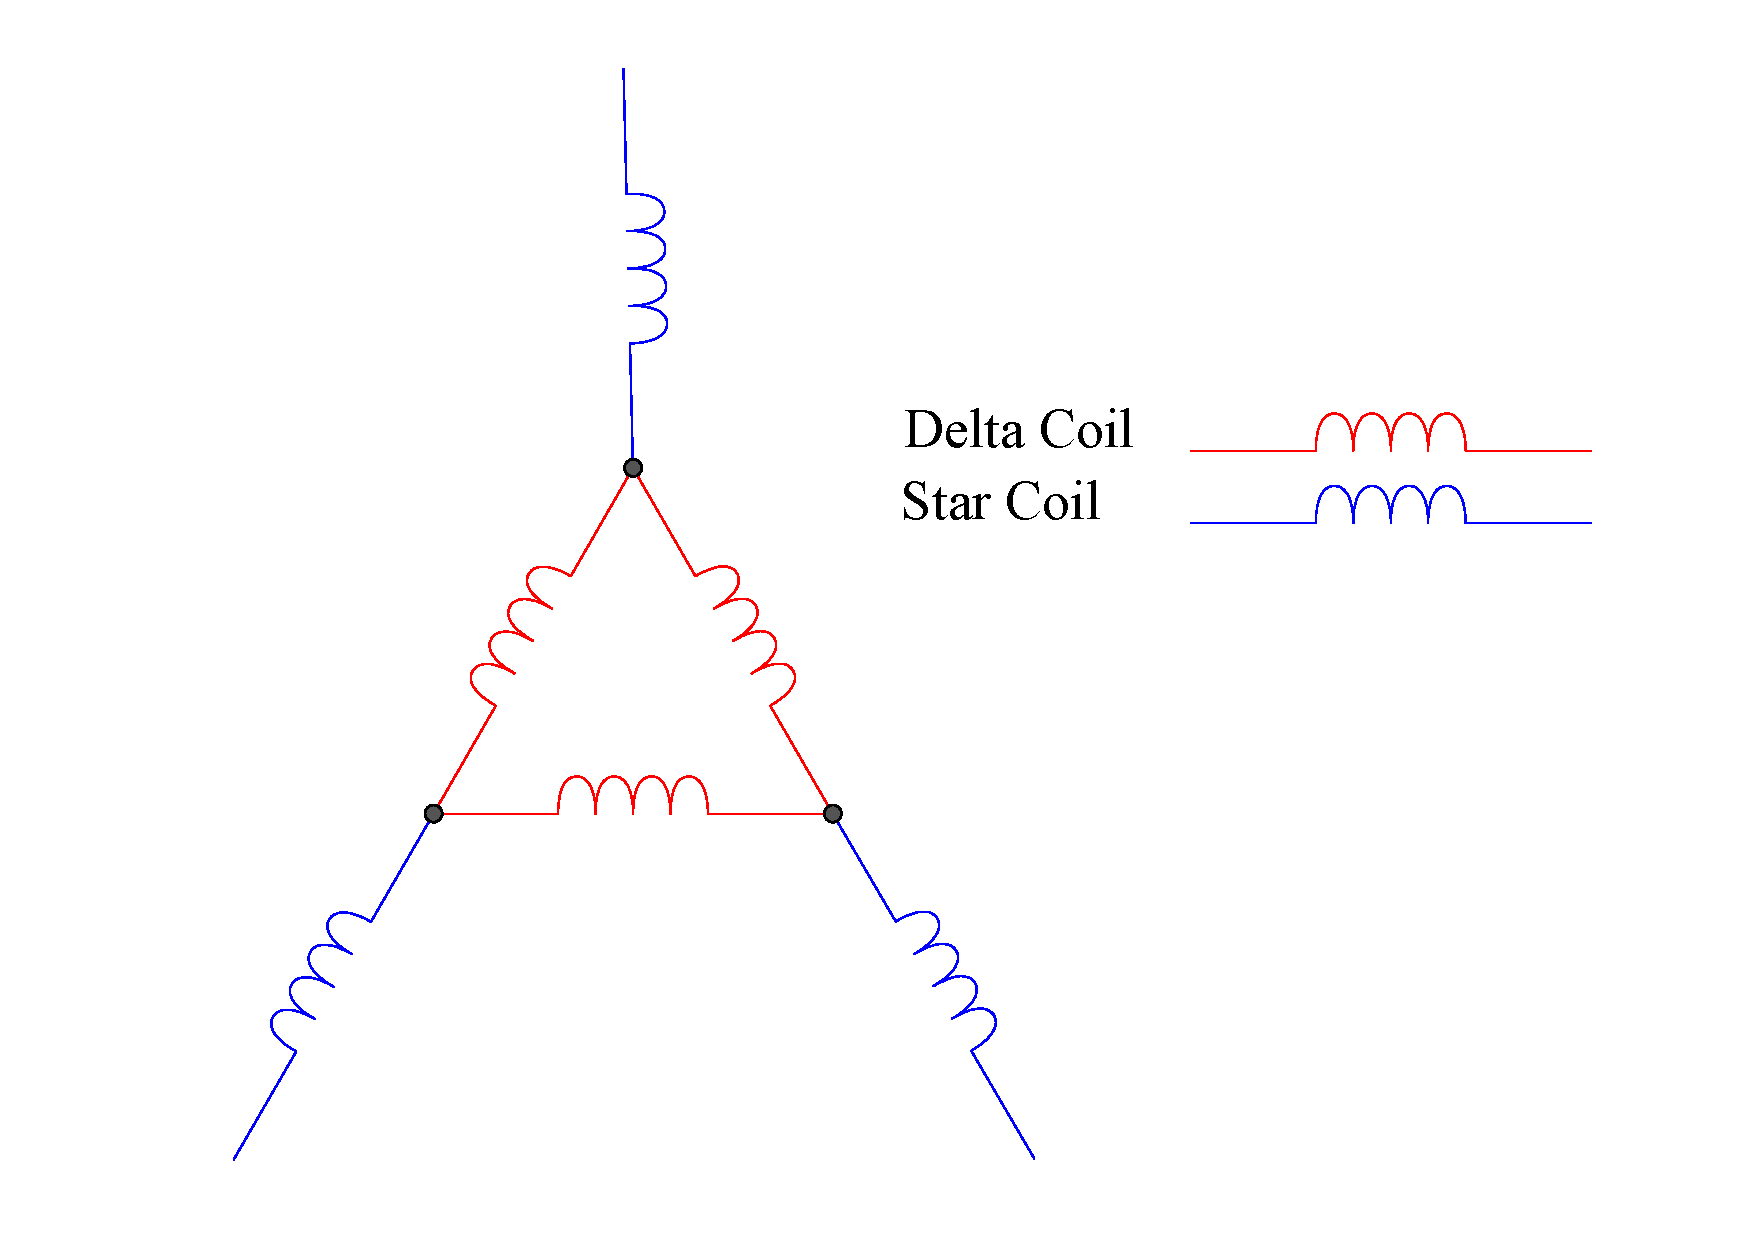
\includegraphics[width=0.75\textwidth]{./../tex/src/pdf/hybrid-star-delta-wiring.pdf} 
            \end{figure}
        \end{minipage}
	

	}
	\frame{
	    \frametitle{Design}
        \techbluetitle{Rotor}
	}

	\frame{
	    \frametitle{Rotor Design}
            \begin{itemize}
                \item internal/external
                \item power factor/wide power range => saliency ratio ($L_d/L_q$)
                \item shape/placement/number of flux bariers
                \item magnets - rare earth (with neodymium/dysprosium), non-rare earth (ferrites)
            \end{itemize}

            \begin{figure}[H]
                \centering
                    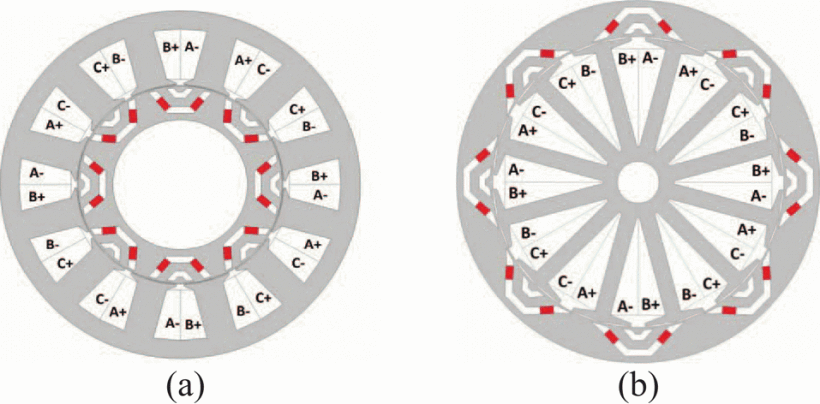
\includegraphics[width=0.75\textwidth]{./../tex/src/png/external-internal-rotor.png} 
            \end{figure}
            
        {\parbox{\linewidth}{\tiny{\color{ctugrey}{BONTHU, Sai Sudheer Reddy; CHOI, Seungdeog; GORGANI, Aida; JANG, Kibong. Design of permanent magnet assisted synchronous reluctance motor with external rotor architecture. In: 2015 IEEE In- ternational Electric Machines \& Drives Conference (IEMDC). Coeur d’Alene, ID: IEEE, 05/2015, pp. 220–226. ISBN 978-1-4799-7941-7. Available from DOI: 10.1109/IEMDC.2015.7409063.}}}}
	}
	\frame{
	    \frametitle{Magnets}
            \begin{itemize}
                \item embedded along the flux barriers, facing the $q$-axis (a) (improvement of torque)
                \item crossing the flux barriers, facing the $d$-axis (b)
            \end{itemize}

            \begin{figure}[H]
                \centering
                    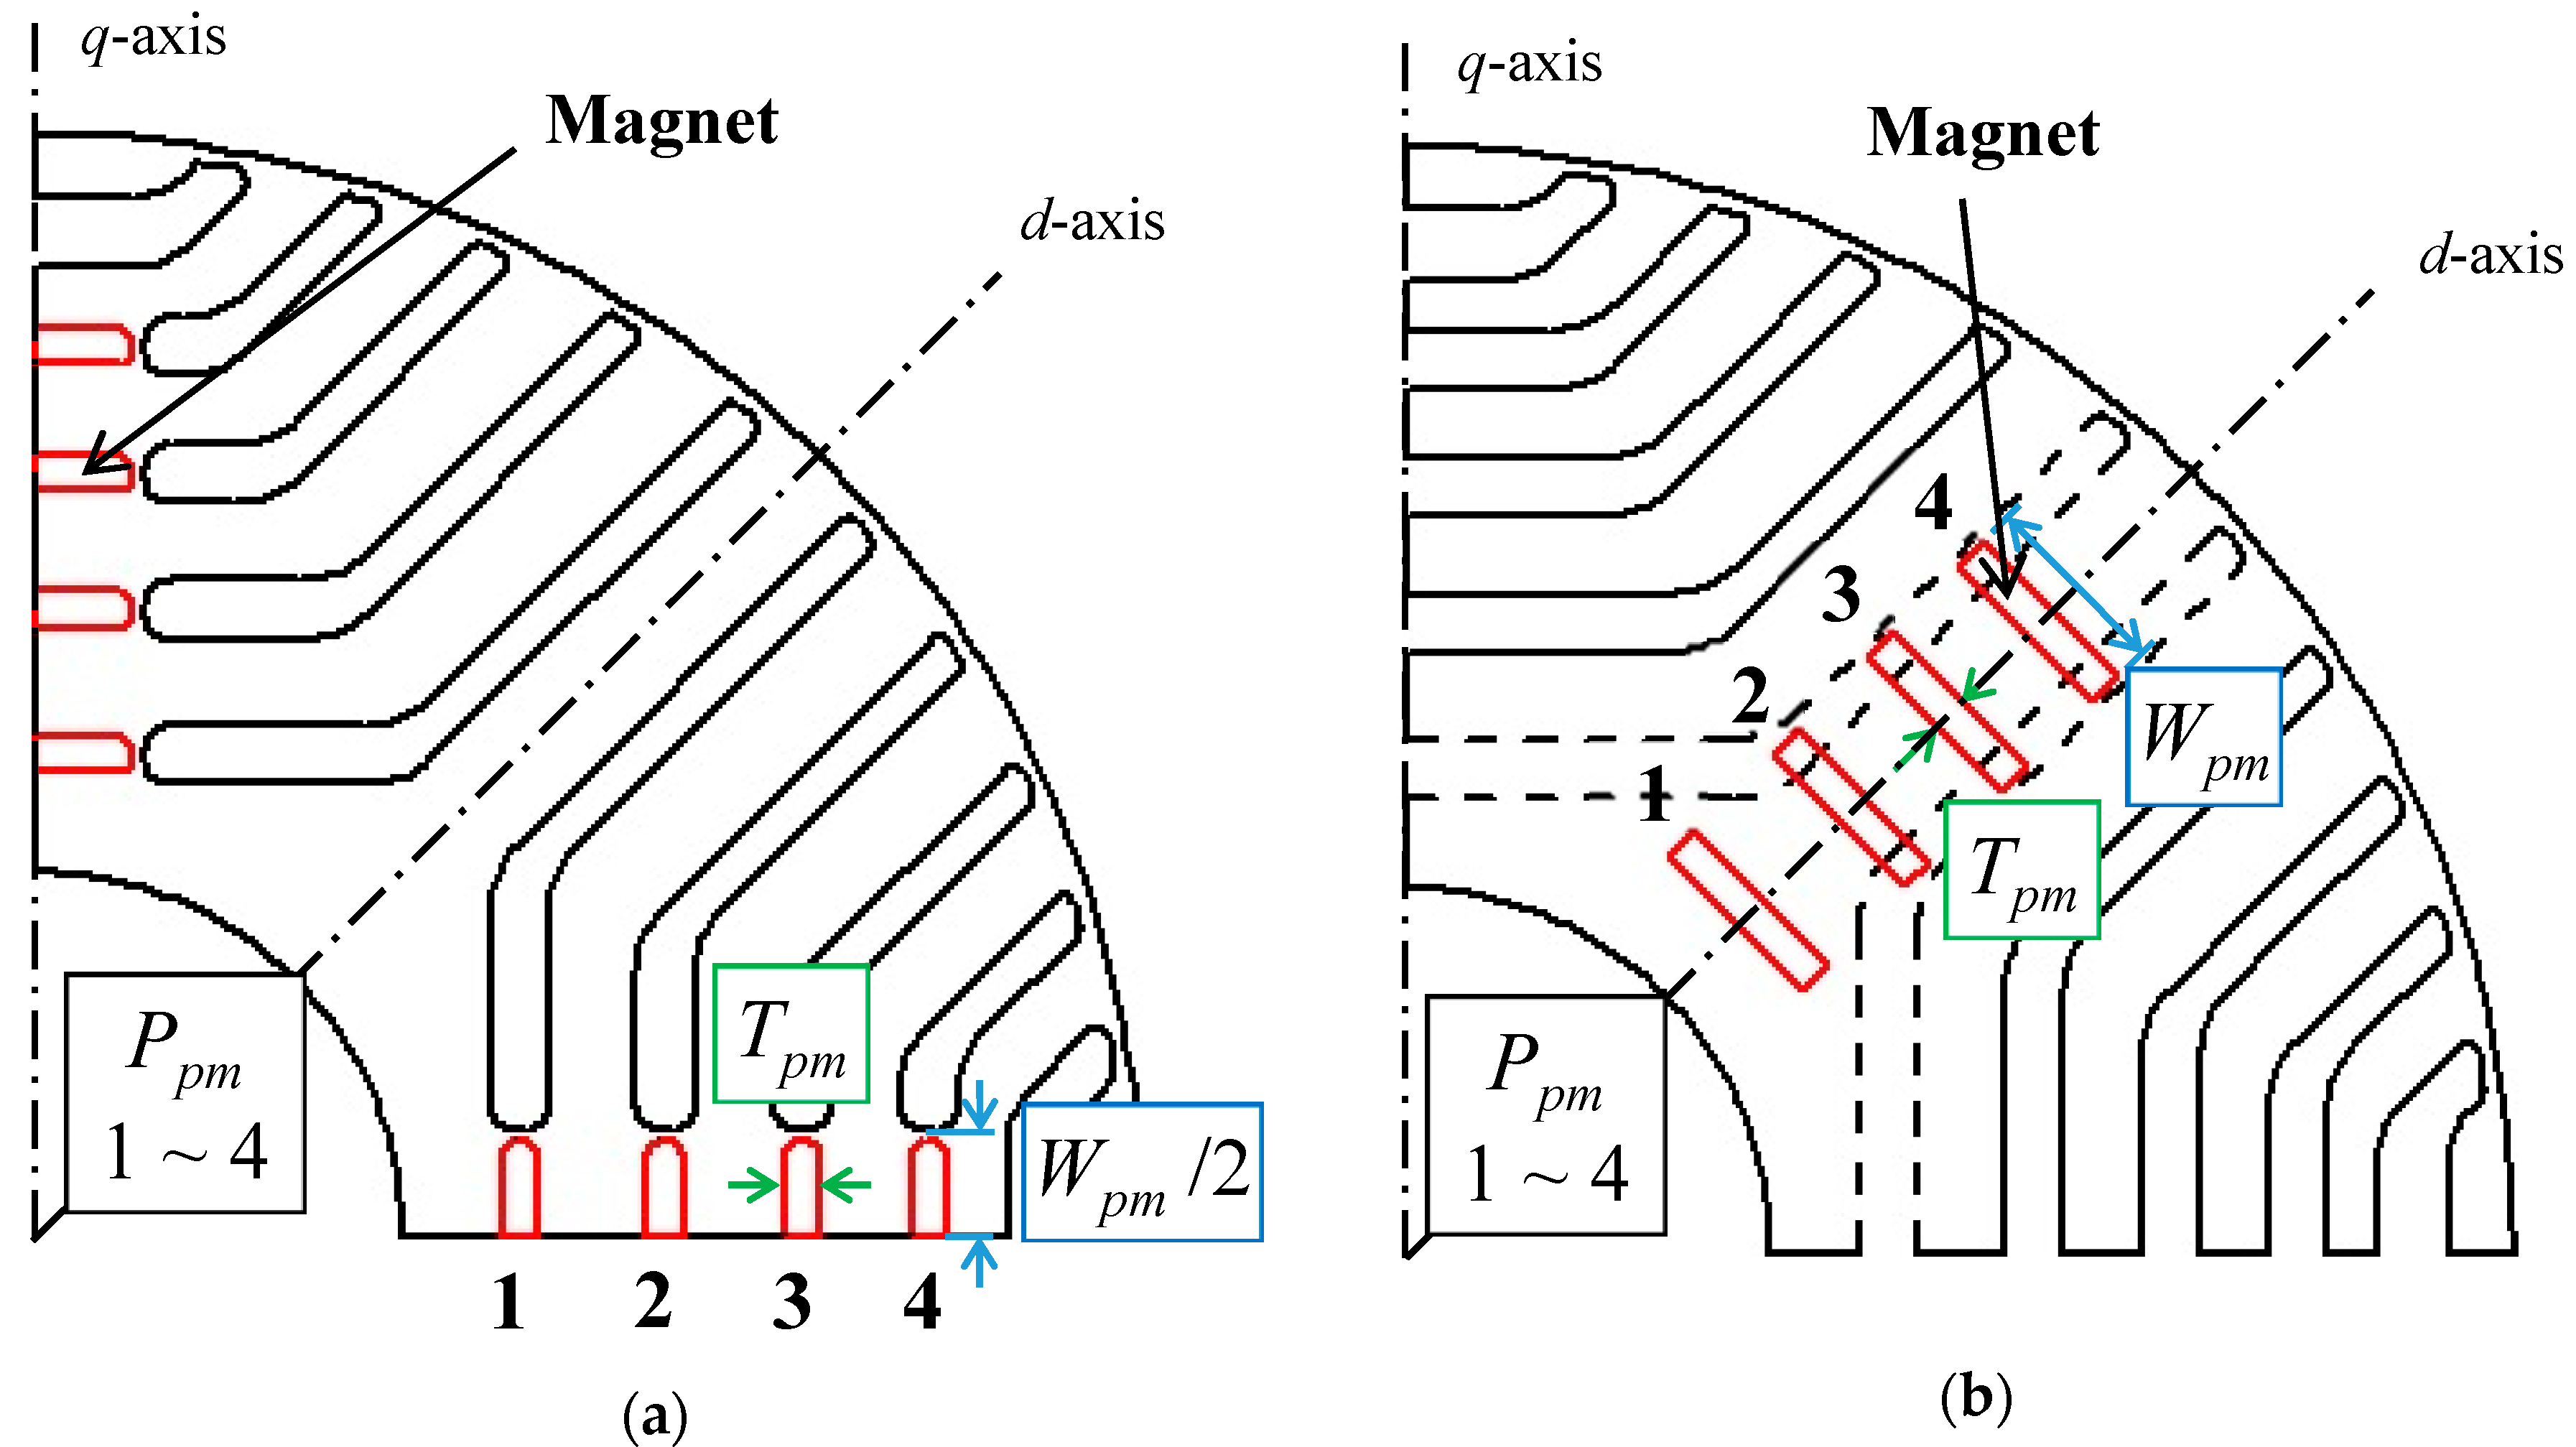
\includegraphics[width=0.75\textwidth]{./../tex/src/png/pmsynrelm-rotor-magnets-position.png} 
            \end{figure}

        {\parbox{\linewidth}{\tiny{\color{ctugrey}{NGO; HSIEH. Performance Analysis of Synchronous Reluctance Motor with Limited Amount of Permanent Magnet. Energies. 09/2019, roč. 12, č. 18, p. 3504. ISSN 1996-1073. Available from DOI: 10.3390/en12183504.}}}}
	}
	\frame{
	    \frametitle{Control}
        \techbluetitle{Control}
	}
	\frame{
	    \frametitle{Control}
            \begin{figure}[H]
                \centering
                    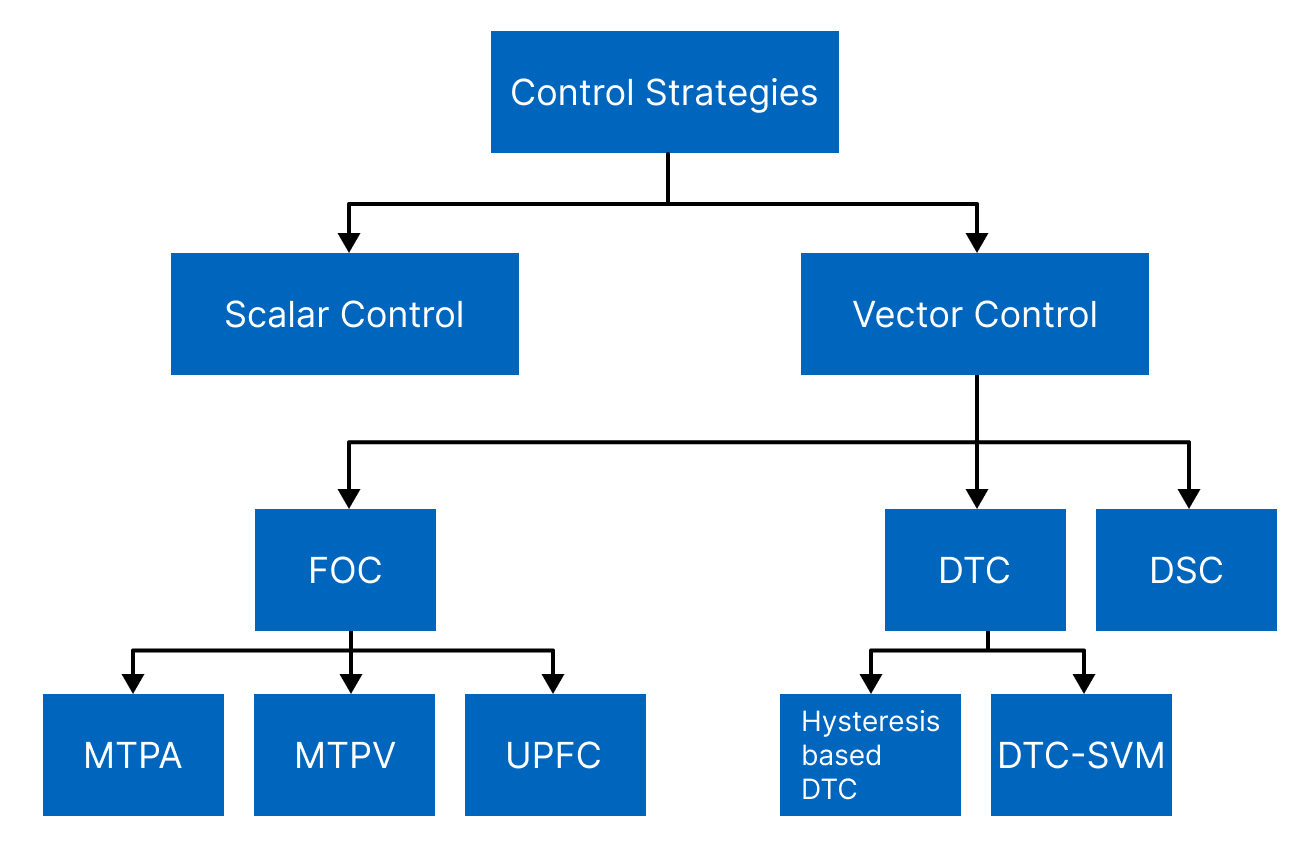
\includegraphics[width=0.75\textwidth]{./../tex/src/png/pmsynrelm-control-strategies.png} 
            \end{figure}
	}
	\frame{
	    \frametitle{Control}
        \vspace*{-1cm}
            \begin{figure}[H]
                \centering
                    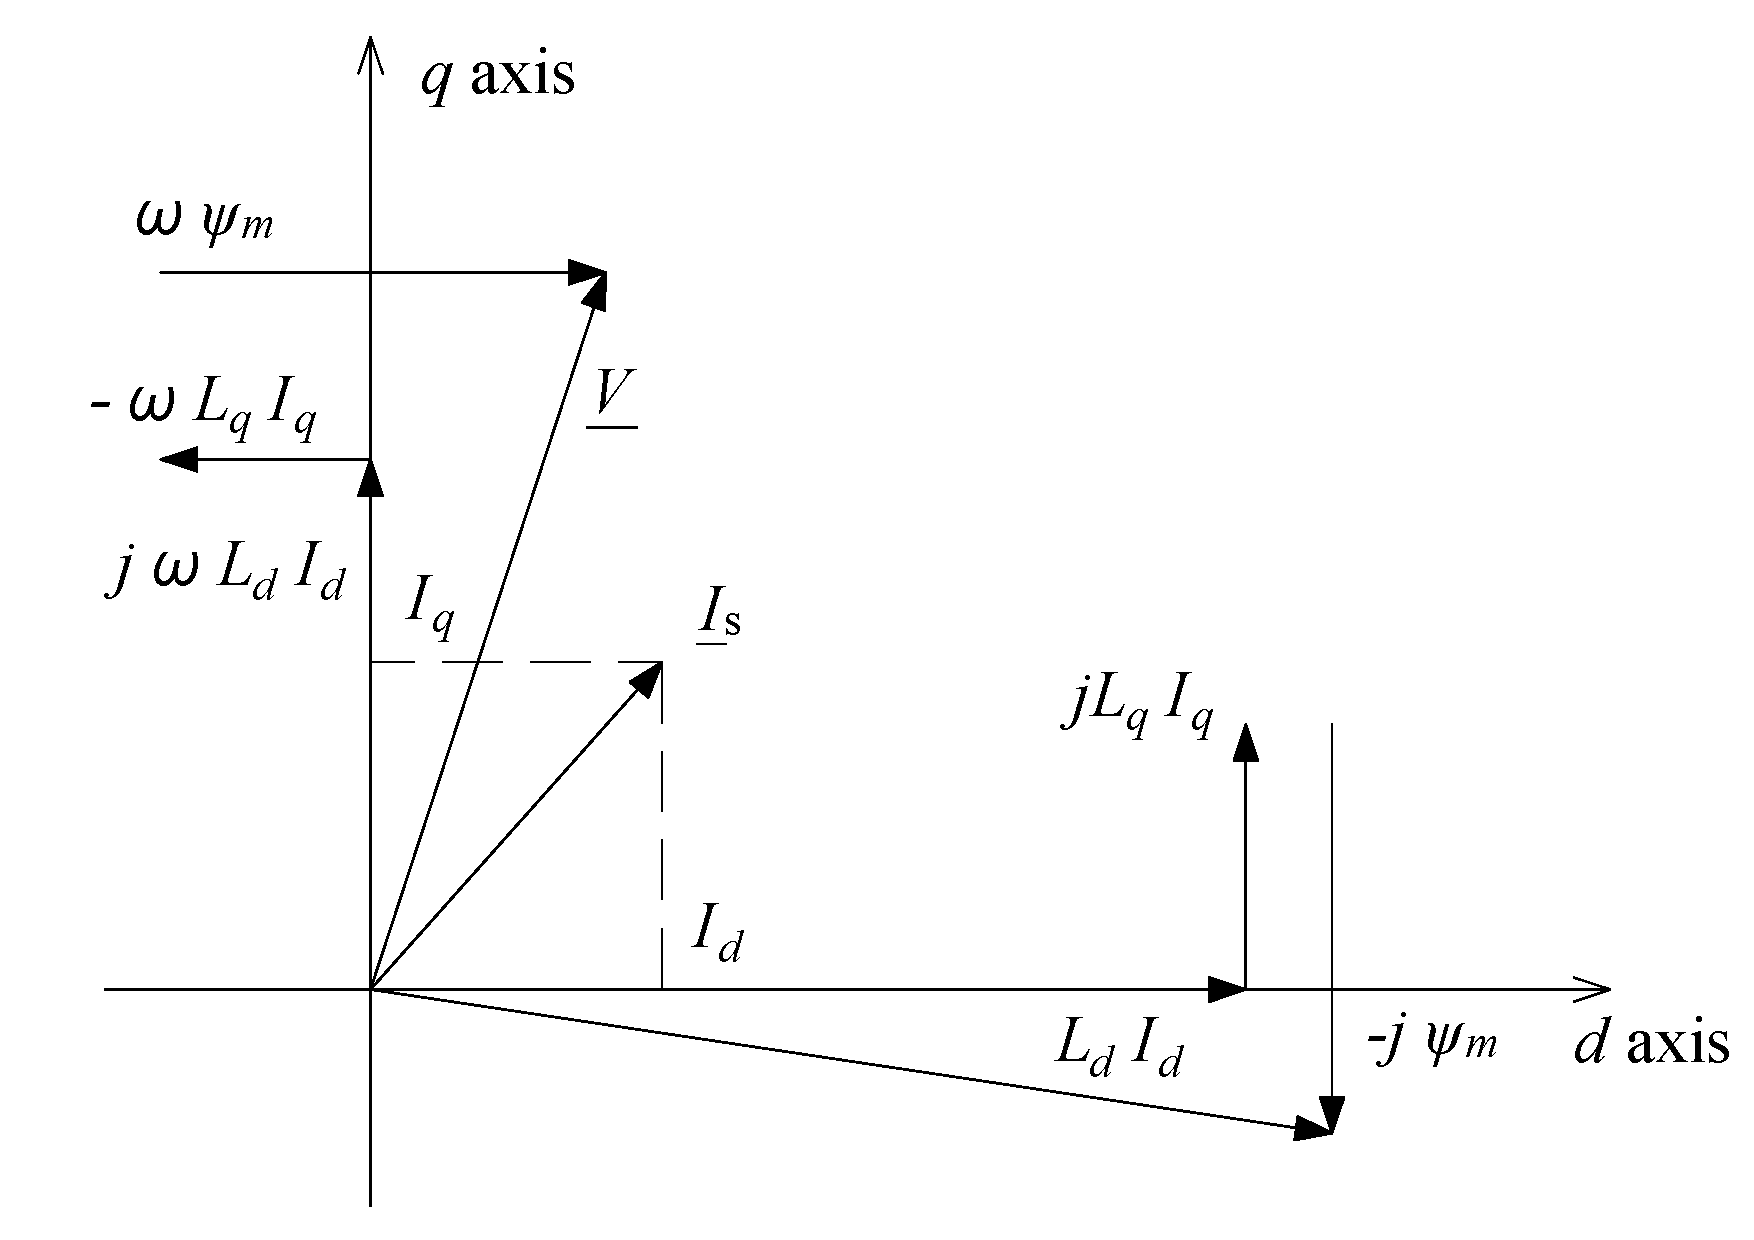
\includegraphics[width=0.75\textwidth]{./../tex/src/pdf/cad-pmasynrm-vector-diagram.pdf} 
            \end{figure}
        \begin{equation}\label{eq:torque-general}
            \begin{gathered}
                T = \frac{3}{2} \text{p}_\text{p} | \underline{\psi_{dq}} \times \underline{i_{dq}} | = \frac{3}{2} \text{p}_\text{p} (\psi_d i_q - \psi_q i_d).
            \end{gathered}
        \end{equation}
        \begin{equation}
            \begin{gathered}
                T = \frac{3}{2} \text{p}_\text{p} (\text{L}_d i_d i_q - (\text{L}_q i_q -\psi_\text{PM}) i_d) = \frac{3}{2} \text{p}_\text{p} (\text{L}_d i_d i_q - \text{L}_q i_q i_d + \psi_\text{PM} i_d).
            \end{gathered}
        \end{equation}
	}
	\frame{
	    \frametitle{Recent research interest}
        {\fontsize{14pt}{14pt}\technikaregular {\color{ctugrey}Recent improvement was achieved:}}\par

        \begin{itemize}
            \item by using non-rare earth materials such as ferrites,
            \item by using novel hybrid stator winding structures,
            \item by analyzing rotor structure types and motor parameters based on the permanent magnet position
and perfecting the design for the specific application,
            \item improving control strategies,
            \item variable flux motor (strategy).
        \end{itemize}
	}
	\frame{
	    \frametitle{XP14DES}
        \techbluetitle{Thank you for your attention.}
	}
\end{document}
